% Options for packages loaded elsewhere
\PassOptionsToPackage{unicode}{hyperref}
\PassOptionsToPackage{hyphens}{url}
%
\documentclass[
]{article}
\usepackage{amsmath,amssymb}
\usepackage{iftex}
\ifPDFTeX
  \usepackage[T1]{fontenc}
  \usepackage[utf8]{inputenc}
  \usepackage{textcomp} % provide euro and other symbols
\else % if luatex or xetex
  \usepackage{unicode-math} % this also loads fontspec
  \defaultfontfeatures{Scale=MatchLowercase}
  \defaultfontfeatures[\rmfamily]{Ligatures=TeX,Scale=1}
\fi
\usepackage{lmodern}
\ifPDFTeX\else
  % xetex/luatex font selection
\fi
% Use upquote if available, for straight quotes in verbatim environments
\IfFileExists{upquote.sty}{\usepackage{upquote}}{}
\IfFileExists{microtype.sty}{% use microtype if available
  \usepackage[]{microtype}
  \UseMicrotypeSet[protrusion]{basicmath} % disable protrusion for tt fonts
}{}
\makeatletter
\@ifundefined{KOMAClassName}{% if non-KOMA class
  \IfFileExists{parskip.sty}{%
    \usepackage{parskip}
  }{% else
    \setlength{\parindent}{0pt}
    \setlength{\parskip}{6pt plus 2pt minus 1pt}}
}{% if KOMA class
  \KOMAoptions{parskip=half}}
\makeatother
\usepackage{xcolor}
\usepackage[margin=1in]{geometry}
\usepackage{graphicx}
\makeatletter
\def\maxwidth{\ifdim\Gin@nat@width>\linewidth\linewidth\else\Gin@nat@width\fi}
\def\maxheight{\ifdim\Gin@nat@height>\textheight\textheight\else\Gin@nat@height\fi}
\makeatother
% Scale images if necessary, so that they will not overflow the page
% margins by default, and it is still possible to overwrite the defaults
% using explicit options in \includegraphics[width, height, ...]{}
\setkeys{Gin}{width=\maxwidth,height=\maxheight,keepaspectratio}
% Set default figure placement to htbp
\makeatletter
\def\fps@figure{htbp}
\makeatother
\setlength{\emergencystretch}{3em} % prevent overfull lines
\providecommand{\tightlist}{%
  \setlength{\itemsep}{0pt}\setlength{\parskip}{0pt}}
\setcounter{secnumdepth}{5}
\usepackage{booktabs}
\usepackage{longtable}
\usepackage{array}
\usepackage{multirow}
\usepackage{wrapfig}
\usepackage{float}
\usepackage{colortbl}
\usepackage{pdflscape}
\usepackage{tabu}
\usepackage{threeparttable}
\usepackage{threeparttablex}
\usepackage[normalem]{ulem}
\usepackage{makecell}
\usepackage{xcolor}
\ifLuaTeX
  \usepackage{selnolig}  % disable illegal ligatures
\fi
\usepackage[]{natbib}
\bibliographystyle{plainnat}
\usepackage{bookmark}
\IfFileExists{xurl.sty}{\usepackage{xurl}}{} % add URL line breaks if available
\urlstyle{same}
\hypersetup{
  pdftitle={Phantom-Words with simultaneous visual presentation - Results},
  pdfkeywords={Keywords},
  hidelinks,
  pdfcreator={LaTeX via pandoc}}

\title{Phantom-Words with simultaneous visual presentation - Results}
\author{Ansgar D. Endress\\
City, University of London}
\date{}

\begin{document}
\maketitle
\begin{abstract}
Abstract (to be written)
\end{abstract}

\section{Predictions}\label{predictions}

The predictions for the current experiment were unclear. On the one
hand, it is plausible that observers might encode entire scenes when
they are presented simultaneously. If so, they should not accept
phantom-words. On the other hand, statistical learning might operate
similarly for simultaneous as for sequential presentation. If so, the
results with sequential presentations should be replicated, especially
because the shapes appear as distinct individual shapes rather than
wholes. Further, presenting the shapes as whole in an object (i.e., in
the white on black presentation) might encourage observers to process
the combination of shapes as a single hole, leading to the rejection of
phantom words.

REMOVED INTERACTION TERM IN GLMM

MAKE SEPARATE TABLES FOR GLMMS

\section{Analysis}\label{analysis}

\subsection{Demographics}\label{demographics}

The main experiment recruited participants from testable minds
(\url{https://minds.testable.org/}). I pilot experiment recruited
participants from first year students at City, University of London
(UK). In the latter population, other experiments typically need to
exclude 30\% to 50\% of the sample due to insufficient attention.
Unfortunately, the present experiment does not offer a clear
performance-based criterion to make sure that participants paid
attention to the stimuli, as the task might be genuinely difficult.
However, given that our main interest lies in the performance on trials
involving phantom-words for participants who succeeded in the
statistical learning task, it is more conservative to exclude
participants whom might not have paid attention to the task, even if
this overestimates the statistical learning abilities.

As a result, I rely on the assumption that earlier statistical learning
literature has shown that participants can learn statistical relations
\emph{in principle}, and exclude those participants not exceeding an
accuracy of 50\% on word vs.~part-word trials. This criterion led to the
removal of 23 and 53 participants from the students and testable
samples, respectively.

The pattern of significance was very similar when all participants were
excluded, with the following differences. First, for the testable minds
sample, performance on the words vs.~part-words trials was no longer
greater than on the phantom-words vs part-words trials, both when shapes
were presented in black on a white background and when the polarity was
inverted. Given that earlier, sequential experiments involving
phantom-words showed equivalent performance for both trial types,
excluding participants is thus more conservative for the current
purposes. Second, for the student sample, the performance difference
between these trial types also ceased to be significant when all
participants are included. Further, when items were presented as black
shapes on white background, there was no significant preference for
words over part-words, suggesting that some of these participants did
not pay attention to the experiment.

The demographics of the remaining participants is given in Table
\ref{tab:vsl-simultaneous-fa-demographics}; age and gender were not
recorded due to experimenter error.

\begin{table}

\caption{\label{tab:vsl-simultaneous-fa-demographics}Demographics of the final sample, after excluding participants whose accuracy on word vs. part-words trials was below 50 percent. For the student population, age and gender have not been recorded due to experimenter error.}
\centering
\begin{tabular}[t]{llrrrrrl}
\toprule
Population & Color polarity & N & Females & Males & Other & Age & Age range\\
\midrule
testable & black on white & 57 & 32 & 25 & 0 & 30.7 & 19-59\\
testable & white on black & 51 & 22 & 29 & 0 & 31.9 & 18-57\\
students & black on white & 12 & 0 & 0 & 12 &  & Inf--Inf\\
students & white on black & 15 & 0 & 0 & 15 &  & Inf--Inf\\
\bottomrule
\end{tabular}
\end{table}

\subsection{Analysis by accuracy}\label{analysis-by-accuracy}

We will analyze the results using two types of analyses. First, I
compare the performance in the different trial types to the chance level
of 50\% using Wilcoxon test. To compare performance across trial types,
I calculate normalized difference scores, that is,
\(\frac{\text{accuracy}_{\text{trial type 1}} - \text{accuracy}_{\text{trial type 2}}}{\text{accuracy}_{\text{trial type 1}} + \text{accuracy}_{\text{trial type 2}}}\).
These difference scores are the compared to the chance level of zero,
again using Wilcoxon tests. I also ask whether any of these results is
affected by the color polarity type (i.e., black on white vs.~white on
black).

Second, we will confirm these results using a set of generalized linear
models.

\begin{table}

\caption{\label{tab:vsl-simultaneous-fa-descriptives}Descriptives of accuracy scores and difference scores, after exclusion of participants whose performance was below 50 percent on word vs. part-word trials. The p value reflects a Wilcoxon test against the chance levels of 50 percent and of 0 for accuracies and difference scores, respectively. The effect of color polarity represents a Wilcoxon test comparing all of these dependent variables as a function of color polarity}
\centering
\begin{tabular}[t]{lrrr}
\toprule
test.type & M & SE & p.wilcox\\
\midrule
\addlinespace[0.3em]
\multicolumn{4}{l}{\textbf{testable - black.on.white (N = 57)}}\\
\hspace{1em}w.pw & 69.152 & 1.395 & 0.000\\
\hspace{1em}w.phw & 49.269 & 2.065 & 0.905\\
\hspace{1em}phw.pw & 58.626 & 1.985 & 0.000\\
\hspace{1em}d.relative.w.pw.w.phw & 0.182 & 0.021 & 0.000\\
\hspace{1em}d.relative.w.pw.ph.pw & 0.091 & 0.021 & 0.000\\
\addlinespace[0.3em]
\multicolumn{4}{l}{\textbf{testable - white.on.black (N = 51)}}\\
\hspace{1em}w.pw & 69.118 & 1.496 & 0.000\\
\hspace{1em}w.phw & 49.346 & 2.012 & 0.985\\
\hspace{1em}phw.pw & 63.562 & 2.516 & 0.000\\
\hspace{1em}d.relative.w.pw.w.phw & 0.178 & 0.021 & 0.000\\
\hspace{1em}d.relative.w.pw.ph.pw & 0.056 & 0.021 & 0.026\\
\addlinespace[0.3em]
\multicolumn{4}{l}{\textbf{testable - zEffect of color polarity}}\\
\hspace{1em}w.pw &  &  & 0.959\\
\hspace{1em}w.phw &  &  & 0.878\\
\hspace{1em}phw.pw &  &  & 0.125\\
\hspace{1em}d.relative.w.pw.w.phw &  &  & 0.784\\
\hspace{1em}d.relative.w.pw.ph.pw &  &  & 0.331\\
\addlinespace[0.3em]
\multicolumn{4}{l}{\textbf{students - black.on.white (N = 12)}}\\
\hspace{1em}w.pw & 67.361 & 2.262 & 0.002\\
\hspace{1em}w.phw & 52.778 & 5.392 & 0.623\\
\hspace{1em}phw.pw & 47.917 & 4.167 & 0.765\\
\hspace{1em}d.relative.w.pw.w.phw & 0.141 & 0.051 & 0.019\\
\hspace{1em}d.relative.w.pw.ph.pw & 0.180 & 0.045 & 0.004\\
\addlinespace[0.3em]
\multicolumn{4}{l}{\textbf{students - white.on.black (N = 15)}}\\
\hspace{1em}w.pw & 66.667 & 2.381 & 0.001\\
\hspace{1em}w.phw & 50.556 & 5.355 & 0.875\\
\hspace{1em}phw.pw & 60.556 & 1.968 & 0.002\\
\hspace{1em}d.relative.w.pw.w.phw & 0.165 & 0.058 & 0.018\\
\hspace{1em}d.relative.w.pw.ph.pw & 0.047 & 0.029 & 0.143\\
\addlinespace[0.3em]
\multicolumn{4}{l}{\textbf{students - zEffect of color polarity}}\\
\hspace{1em}w.pw &  &  & 0.698\\
\hspace{1em}w.phw &  &  & 0.825\\
\hspace{1em}phw.pw &  &  & 0.008\\
\hspace{1em}d.relative.w.pw.w.phw &  &  & 0.807\\
\hspace{1em}d.relative.w.pw.ph.pw &  &  & 0.011\\
\bottomrule
\end{tabular}
\end{table}

\begin{figure}

{\centering 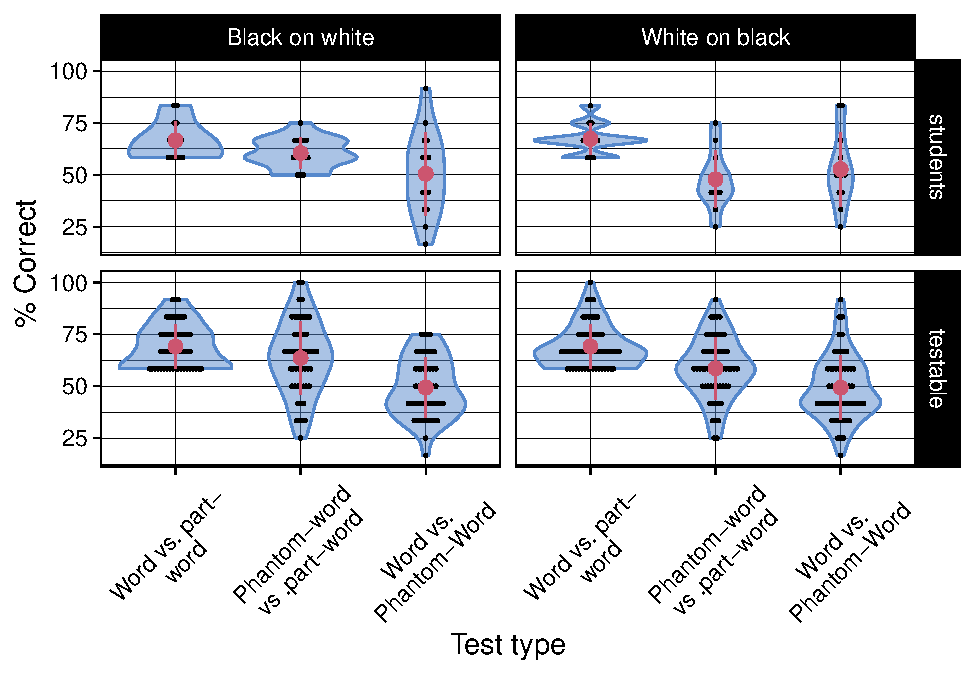
\includegraphics[width=0.8\linewidth]{vsl_phamtoms_simultaneous_results_files/figure-latex/vsl-simultaneous-fa-plot-accuracy-1} 

}

\caption{Accuracy in the different trial types (words vs. part-words, phantom-words vs. part-words, and words vs. phantom-words), after exclusion of participants whose performance was below 50\% in the word vs. part-word trials. The dots, error bars and violion represent the sample averages, 95\% bootstrap confidence intervals and the distribution of the average accuracy for individual participants, respectively. Empty circles represent individual participants.}\label{fig:vsl-simultaneous-fa-plot-accuracy}
\end{figure}

\begin{figure}

{\centering 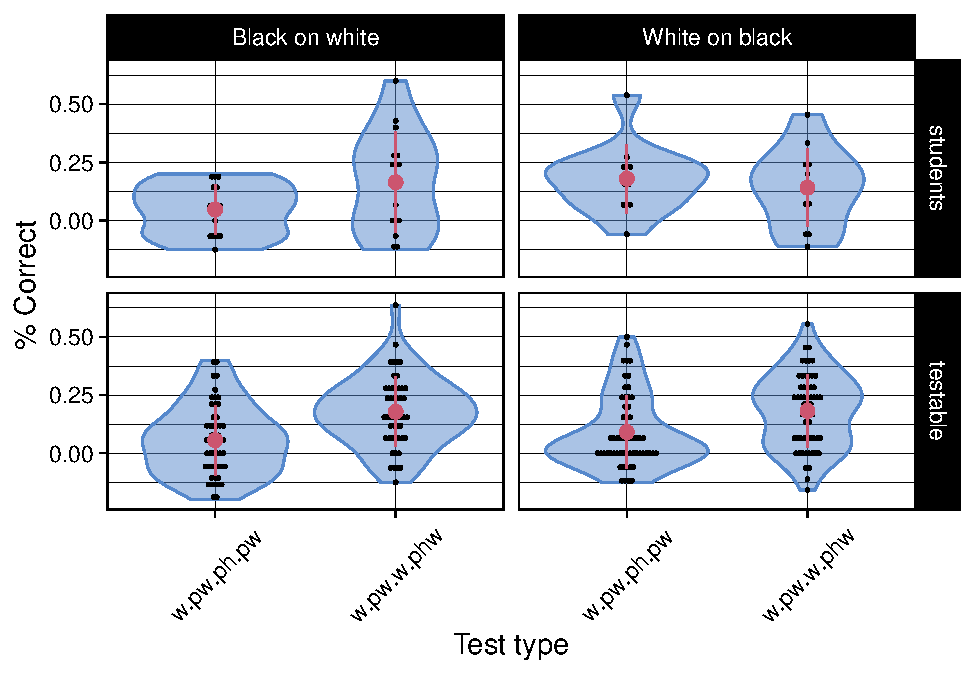
\includegraphics[width=0.8\linewidth]{vsl_phamtoms_simultaneous_results_files/figure-latex/vsl-simultaneous-fa-plot-difference-scores-1} 

}

\caption{Relative difference scores for contrasts between different trial types (word vs. part-word trials vs. phantom-word vs. part-word trials, and word vs. part-word trials vs. word vs. phantom-word trials), after exclusion of participants whose performance was below 50\% in the word vs. part-word trials. The dots, error bars and violion represent the sample averages, 95\% bootstrap confidence intervals and the distribution of the difference scores for individual participants, respectively. Empty circles represent individual participants.}\label{fig:vsl-simultaneous-fa-plot-difference-scores}
\end{figure}

As shown in Table \ref{tab:vsl-simultaneous-fa-descriptives} and Figure
\ref{fig:vsl-simultaneous-fa-plot-accuracy}, participants from the
testable minds sample preferred both words and phantom-words to
part-words. In contrast, the had no preference for words over
phantom-words. Similar results were obtained for both color polarity
types, with no discernible effect of color polarity type. The results
for student sample were similar, except that there was no preference for
phantom-words over part-words when black shapes were presented on a
white background, and that the preference for phantom-words over
part-words was significantly greater when white shapes were presented on
a black background. However, given that the result relied on only 12
participants, I tentatively conclude that the current experiment
replicate \citep{Endress-Phantoms} and \citep{Endress-Phantoms-Vision},
in that phantom-words are preferred to part-words, and there is no
marked preference for words over phantom-words.

To compare performance in the different trial types, I calculated the
difference scores mentioned above. As shown in Table
\ref{tab:vsl-simultaneous-fa-descriptives} and Figure
\ref{fig:vsl-simultaneous-fa-plot-difference-scores}, participants from
the testable sample performed much better on word vs.~part-word trials
than on word vs.~phantom-word trials, irrespective of the color polarity
type. This suggests that participants find discriminations based on TPs
much easier than discriminations based on frequency of occurrence, which
is problematic if statistical learning leads to memory for units.
However, performance was also somewhat better for word vs.~part-word
trials than for phantom-word vs.~part-word trials, suggesting that we
cannot rule out that participants might also have some ability to track
frequencies of occurrence. However, the corresponding difference score
was much smaller than that comparing words vs.~part-word and word
vs.~phantom-word trials, and ceased to be significant when all
participants were included.

In the student sample, results were similar, except that I did not
detect a performance difference between word vs.~part-word and
phantom-word vs.~part-word trials when white shapes were presented on a
black background.

\begin{table}[!h]

\caption{\label{tab:vsl-simultaneous-fa-plot-glmer-correct-calculate-and-print}Results of generalized linear mixed models for trial-by-trial responses, after exclusion of participants whose performance was below 50\% in the word vs. part-word trials.}
\centering
\resizebox{\linewidth}{!}{
\begin{tabular}[t]{lrrlrrlrr}
\toprule
\multicolumn{1}{c}{ } & \multicolumn{3}{c}{Log-odds} & \multicolumn{3}{c}{Odd ratios} & \multicolumn{2}{c}{ } \\
\cmidrule(l{3pt}r{3pt}){2-4} \cmidrule(l{3pt}r{3pt}){5-7}
term & Estimate & SE & CI & Estimate & SE & CI & t & p\\
\midrule
\addlinespace[0.3em]
\multicolumn{9}{l}{\textbf{testable - w.pw vs. w.phw}}\\
\hspace{1em}test.typew.pw & 0.834 & 0.082 & {}[0.674, 0.995] & 2.303 & 0.189 & {}[1.96, 2.7] & 10.190 & 0.000\\
\hspace{1em}color.typewhite.on.black & 0.001 & 0.082 & {}[-0.159, 0.161] & 1.001 & 0.082 & {}[0.853, 1.17] & 0.011 & 0.991\\
\addlinespace[0.3em]
\multicolumn{9}{l}{\textbf{testable - w.pw vs. phw.pw}}\\
\hspace{1em}test.typew.pw & 0.460 & 0.114 & {}[0.237, 0.683] & 1.584 & 0.180 & {}[1.27, 1.98] & 4.047 & 0.000\\
\hspace{1em}color.typewhite.on.black & 0.209 & 0.117 & {}[-0.02, 0.437] & 1.232 & 0.144 & {}[0.98, 1.55] & 1.788 & 0.074\\
\hspace{1em}test.typew.pw:color.typewhite.on.black & -0.210 & 0.166 & {}[-0.536, 0.116] & 0.810 & 0.135 & {}[0.585, 1.12] & -1.263 & 0.207\\
\addlinespace[0.3em]
\multicolumn{9}{l}{\textbf{students - w.pw vs. w.phw}}\\
\hspace{1em}test.typew.pw & 0.646 & 0.163 & {}[0.328, 0.965] & 1.909 & 0.310 & {}[1.39, 2.62] & 3.977 & 0.000\\
\hspace{1em}color.typewhite.on.black & -0.062 & 0.166 & {}[-0.387, 0.263] & 0.940 & 0.156 & {}[0.679, 1.3] & -0.374 & 0.708\\
\addlinespace[0.3em]
\multicolumn{9}{l}{\textbf{students - w.pw vs. phw.pw}}\\
\hspace{1em}test.typew.pw & 0.808 & 0.244 & {}[0.33, 1.29] & 2.243 & 0.547 & {}[1.39, 3.62] & 3.315 & 0.001\\
\hspace{1em}color.typewhite.on.black & 0.512 & 0.226 & {}[0.0691, 0.955] & 1.669 & 0.377 & {}[1.07, 2.6] & 2.266 & 0.023\\
\hspace{1em}test.typew.pw:color.typewhite.on.black & -0.543 & 0.328 & {}[-1.19, 0.0997] & 0.581 & 0.191 & {}[0.305, 1.1] & -1.656 & 0.098\\
\bottomrule
\end{tabular}}
\end{table}

I confirmed these results using generalized linear mixed models with the
fixed factor predictors trial type and and color polarity as well as
their interaction, and a random intercept for participants. I fitted
separate model for each sample (testable vs.~students) and trial
contrast (word vs.~part-word trials vs.~word vs.~phantom-word trials and
word vs.~part-words and phantom-word vs.~part-word trials). The models
showed that performance on word vs.~part-word trials is significantly
better than for word vs.~phantom-word trials. In the testable
population, they also showed that performance on word vs.~part-word
trials was significantly better than on phantom-word vs.~part-word
trials, though this predictor was not significant in the student
population. Further, the odds ratio associated with the former contrast
was almost twice as high as that from the latter contrast.

There were generally no main effects or interactions with polarity type,
though students performed somewhat better for black on white displays.

\section{Discussion}\label{discussion}

\clearpage

\section{Appendix 1: Results with the full
sample}\label{appendix-1-results-with-the-full-sample}

As shown in Table \ref{tab:vsl-simultaneous-fa-descriptives-full-sample}
and Figure \ref{fig:vsl-simultaneous-fa-plot-accuracy-full-sample},
participants from the testable minds sample preferred both words and
phantom-words to part-words. In contrast, the had no preference for
words over phantom-words. Similar results were obtained for both color
polarity types, with no discernible effect of color polarity type. In
the complete student sample, in contrast, the only significant
preference was that for words over part-words, but only when black
shapes were presented on a white background. These contrasting results
presumably reflect the finding that, in other experiments that can
implement attention check manipulations, 30\% to 50\% of such samples
need to be excluded due to insufficient attention.

As a result, I tentatively conclude that, at least in the testable minds
sample, the current experiment replicate \citep{Endress-Phantoms} and
\citep{Endress-Phantoms-Vision}, in that phantom-words are preferred to
part-words, and there is no marked preference for words over
phantom-words.

To compare performance across trial types, I calculated the difference
scores mentioned above. As shown in Table
\ref{tab:vsl-simultaneous-fa-descriptives-full-sample} and Figure
\ref{fig:vsl-simultaneous-fa-plot-difference-scores-full-sample},
participants from the testable sample performed much better on word
vs.~part-word trials than on word vs.~phantom-word trials, irrespective
of the color polarity type. This suggests that participants find
discriminations based on TPs much easier than discriminations based on
frequency of occurrence, which is problematic if statistical learning
leads to memory for units. In contrast to the results with the
restricted sample, performance was not significantly different between
word vs.~part-word trials and phantom-word vs.~part-word trials.

In the student sample, only the comparison between word vs.~part-word
trials and word vs.~phantom-word trials was statistically different from
zero, but only when black shapes were presented on a white background.
However, and as mentioned above, this sample likely contained a sizable
proportion of participants who paid little attention to the stimuli.

I confirmed these results using generalized linear mixed models with the
fixed factor predictors trial type and and color polarity as well as
their interaction, and a random intercept for participants. I fitted
separate model for each sample (testable vs.~students) and trial
contrast (word vs.~part-word trials vs.~word vs.~phantom-word trials and
word vs.~part-words and phantom-word vs.~part-word trials). As shown in
Table
\ref{tab:vsl-simultaneous-fa-plot-glmer-correct-calculate-and-print-full-sample},
the models showed that performance on word vs.~part-word trials is
significantly better than for word vs.~phantom-word trials. In contrast,
there was no difference between word vs part-word and phantom-word
vs.~part-word trials.

There were generally no main effects or interactions with polarity type.

  \bibliography{/Users/endress/ansgar.bib}

\end{document}
